\documentclass{article}

\usepackage{hyperref}
\hypersetup{
	colorlinks=true,
	linkcolor=blue,
	urlcolor=cyan,}
\usepackage{booktabs}
\usepackage{textgreek}

%%%%%%%%%%%%%%%%%%%%%%%%%%%%%%%%%%%%%%%%%
% Lachaise Assignment
% Structure Specification File
% Version 1.0 (26/6/2018)
%
% This template originates from:
% http://www.LaTeXTemplates.com
%
% Authors:
% Marion Lachaise & François Févotte
% Vel (vel@LaTeXTemplates.com)
%
% License:
% CC BY-NC-SA 3.0 (http://creativecommons.org/licenses/by-nc-sa/3.0/)
% 
%%%%%%%%%%%%%%%%%%%%%%%%%%%%%%%%%%%%%%%%%

%----------------------------------------------------------------------------------------
%	PACKAGES AND OTHER DOCUMENT CONFIGURATIONS
%----------------------------------------------------------------------------------------

\usepackage{amsmath,amsfonts,stmaryrd,amssymb} % Math packages

\usepackage{enumerate} % Custom item numbers for enumerations

\usepackage[ruled]{algorithm2e} % Algorithms

\usepackage[framemethod=tikz]{mdframed} % Allows defining custom boxed/framed environments

\usepackage{listings} % File listings, with syntax highlighting
\lstset{
	basicstyle=\ttfamily, % Typeset listings in monospace font
}

%----------------------------------------------------------------------------------------
%	DOCUMENT MARGINS
%----------------------------------------------------------------------------------------

\usepackage{geometry} % Required for adjusting page dimensions and margins

\geometry{
	paper=a4paper, % Paper size, change to letterpaper for US letter size
	top=2.5cm, % Top margin
	bottom=3cm, % Bottom margin
	left=2.5cm, % Left margin
	right=2.5cm, % Right margin
	headheight=14pt, % Header height
	footskip=1.5cm, % Space from the bottom margin to the baseline of the footer
	headsep=1.2cm, % Space from the top margin to the baseline of the header
	%showframe, % Uncomment to show how the type block is set on the page
}

%----------------------------------------------------------------------------------------
%	FONTS
%----------------------------------------------------------------------------------------

\usepackage[utf8]{inputenc} % Required for inputting international characters
\usepackage[T1]{fontenc} % Output font encoding for international characters

\usepackage{XCharter} % Use the XCharter fonts

%----------------------------------------------------------------------------------------
%	COMMAND LINE ENVIRONMENT
%----------------------------------------------------------------------------------------

% Usage:
% \begin{commandline}
%	\begin{verbatim}
%		$ ls
%		
%		Applications	Desktop	...
%	\end{verbatim}
% \end{commandline}

\mdfdefinestyle{commandline}{
	leftmargin=10pt,
	rightmargin=10pt,
	innerleftmargin=15pt,
	middlelinecolor=black!50!white,
	middlelinewidth=2pt,
	frametitlerule=false,
	backgroundcolor=black!5!white,
	frametitle={Command Line},
	frametitlefont={\normalfont\sffamily\color{white}\hspace{-1em}},
	frametitlebackgroundcolor=black!50!white,
	nobreak,
}

% Define a custom environment for command-line snapshots
\newenvironment{commandline}{
	\medskip
	\begin{mdframed}[style=commandline]
}{
	\end{mdframed}
	\medskip
}

%----------------------------------------------------------------------------------------
%	FILE CONTENTS ENVIRONMENT
%----------------------------------------------------------------------------------------

% Usage:
% \begin{file}[optional filename, defaults to "File"]
%	File contents, for example, with a listings environment
% \end{file}

\mdfdefinestyle{file}{
	innertopmargin=1.6\baselineskip,
	innerbottommargin=0.8\baselineskip,
	topline=false, bottomline=false,
	leftline=false, rightline=false,
	leftmargin=2cm,
	rightmargin=2cm,
	singleextra={%
		\draw[fill=black!10!white](P)++(0,-1.2em)rectangle(P-|O);
		\node[anchor=north west]
		at(P-|O){\ttfamily\mdfilename};
		%
		\def\l{3em}
		\draw(O-|P)++(-\l,0)--++(\l,\l)--(P)--(P-|O)--(O)--cycle;
		\draw(O-|P)++(-\l,0)--++(0,\l)--++(\l,0);
	},
	nobreak,
}

% Define a custom environment for file contents
\newenvironment{file}[1][File]{ % Set the default filename to "File"
	\medskip
	\newcommand{\mdfilename}{#1}
	\begin{mdframed}[style=file]
}{
	\end{mdframed}
	\medskip
}

%----------------------------------------------------------------------------------------
%	NUMBERED QUESTIONS ENVIRONMENT
%----------------------------------------------------------------------------------------

% Usage:
% \begin{question}[optional title]
%	Question contents
% \end{question}

\mdfdefinestyle{question}{
	innertopmargin=1.2\baselineskip,
	innerbottommargin=0.8\baselineskip,
	roundcorner=5pt,
	nobreak,
	singleextra={%
		\draw(P-|O)node[xshift=1em,anchor=west,fill=white,draw,rounded corners=5pt]{%
		Question \theQuestion\questionTitle};
	},
}

\newcounter{Question} % Stores the current question number that gets iterated with each new question

% Define a custom environment for numbered questions
\newenvironment{question}[1][\unskip]{
	\bigskip
	\stepcounter{Question}
	\newcommand{\questionTitle}{~#1}
	\begin{mdframed}[style=question]
}{
	\end{mdframed}
	\medskip
}

%----------------------------------------------------------------------------------------
%	WARNING TEXT ENVIRONMENT
%----------------------------------------------------------------------------------------

% Usage:
% \begin{warn}[optional title, defaults to "Warning:"]
%	Contents
% \end{warn}

\mdfdefinestyle{warning}{
	topline=false, bottomline=false,
	leftline=false, rightline=false,
	nobreak,
	singleextra={%
		\draw(P-|O)++(-0.5em,0)node(tmp1){};
		\draw(P-|O)++(0.5em,0)node(tmp2){};
		\fill[black,rotate around={45:(P-|O)}](tmp1)rectangle(tmp2);
		\node at(P-|O){\color{white}\scriptsize\bf !};
		\draw[very thick](P-|O)++(0,-1em)--(O);%--(O-|P);
	}
}

% Define a custom environment for warning text
\newenvironment{warn}[1][Warning:]{ % Set the default warning to "Warning:"
	\medskip
	\begin{mdframed}[style=warning]
		\noindent{\textbf{#1}}
}{
	\end{mdframed}
}

%----------------------------------------------------------------------------------------
%	INFORMATION ENVIRONMENT
%----------------------------------------------------------------------------------------

% Usage:
% \begin{info}[optional title, defaults to "Info:"]
% 	contents
% 	\end{info}

\mdfdefinestyle{info}{%
	topline=false, bottomline=false,
	leftline=false, rightline=false,
	nobreak,
	singleextra={%
		\fill[black](P-|O)circle[radius=0.4em];
		\node at(P-|O){\color{white}\scriptsize\bf i};
		\draw[very thick](P-|O)++(0,-0.8em)--(O);%--(O-|P);
	}
}

% Define a custom environment for information
\newenvironment{info}[1][Info:]{ % Set the default title to "Info:"
	\medskip
	\begin{mdframed}[style=info]
		\noindent{\textbf{#1}}
}{
	\end{mdframed}
}
 % Include the file specifying the document structure and custom commands

%----------------------------------------------------------------------------------------
%	ASSIGNMENT INFORMATION
%----------------------------------------------------------------------------------------

\title{Week 6: Electrocardiography (ECG) II}
\author{BIOE 320 Systems Physiology Laboratory} 
\date{}
%----------------------------------------------------------------------------------------

\begin{document}
\large
\maketitle

\section*{Objectives}
\begin{enumerate}
	\item To record ECG measurements from leads I and III in the following conditions: lying down, sitting up, and breathing deeply while sitting.
	\item To use Einthoven's Law to estimate the mean electrical axis and magnitude of the QRS complex.
\end{enumerate}

\section*{Background}


\subsection*{Electrical Activity of the Heart (Review)}
\begin{figure}[h]
\centering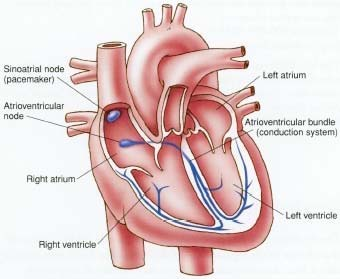
\includegraphics[width=0.4\textwidth]{../images/ECG_II_1a.jpg}
\centering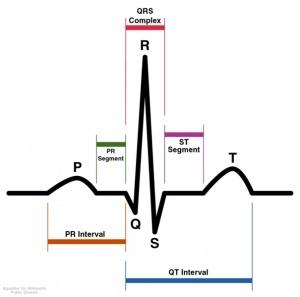
\includegraphics[width=0.3\textwidth]{../images/ECG_II_1b.jpg}
\caption{The pacemaker system and the PQRST wave}
\label{pacemaker}
\end{figure}

The heart's electrical system begins at the sinoatrial (SA) node, the primary pacemaker of the heart, where electric potential originates. The polarization spreads throughout the atria, initiating contraction of atrial myocardium (P wave of ECG). The signal then travels to the AV node where it is delayed, allowing time for the blood to leave the atria before ventricular contraction begins. After the AV nodes, the signal is conducted down the left and right bundle branches and the Purkinje fibers to the ventricular myocardium. Depolarization of the ventricles is recorded as the QRS complex in the ECG, and repolarization of the ventricles is recorded as the T wave. This process is summarized in Fig. \ref{pacemaker}. In the last lab, we saw how the heart's electrical activity can be analyzed using an ECG (specifically, the standard bipolar lead II). This week, we will explore how to interpret the magnitude and direction of the ECG signal and how to estimate the mean electrical axis of the QRS complex.

\subsection*{Einthoven's Law}
ECGs are produced by a system of leads attached to the body. One common lead system uses the three standard bipolar limb leads. The electrode placement defines the recorded direction of the lead, when going from the negative to the positive electrode. The ECG is read as the computed difference (magnitude) between the positive and negative electrodes as a change in voltage over time.\\

The standard bipolar lim leads, their polarity, and axes are as follows:
\begin{table}[h]
	\centering
	\begin{tabular}[h!]{ccc}
	\toprule
	Lead & Polarity & Lead Axis\\
	\midrule
	Lead I & right arm (-) to left arm (+) & 180\textdegree\ to 0\textdegree\\
	 Lead II & right arm (-) to left leg (+) & -120\textdegree\ to 60\textdegree\\
	 Lead III & left arm (-) to left leg (+) & -60\textdegree\ to 120\textdegree\\
	\bottomrule
	\end{tabular}
	\end{table}

The placement of the leads is the result of the extension of Einthoven's Triangle, a triangle of three leads that surrounds the heart. The ECG for each lead displays the amplitude of the voltage as projected onto that lead. To determine the value closest to the actual direction of the heart, Lead II is usually used. However, because the three leads are connected in a loop, Kirchoff's Voltage Law (KVL) states that the voltage drop around the loop must be equal to zero, and therefore, Einthoven's Law can be used to determine the value of one lead if we know the value of the other two.

\subsection*{Mean Electrical Axis: Direction}
During the cardiac cycle, the current spreads along specialized pathways, depolarizing the heart in a specific sequence. Consequently, the electrical activity has .directionality, that is, a spatial orientation represented by an electrical axis. The summation of all the vectors occurring in a cardiac cycle (i.e. the preponderant direction of current flow during the cardiac cycle) is called the mean electrical axis (Fig. \ref{axis})

\begin{figure}[h]
\centering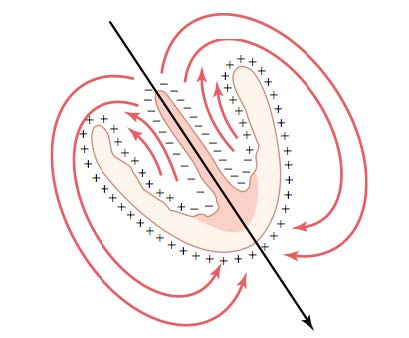
\includegraphics[width=0.5\textwidth]{../images/ECG_II_2.jpg}
\caption{Mean vector through partially depolarized ventricles}
\label{axis}
\end{figure}

Since the QRS complex caused by ventricular depolarization represents the majority of the electrical activity of the heart, you can approximate the mean electrical axis by looking only in this interval. Typically, in an adult, the mean electrical axis lies along a line extending from the base of the apex of the heart and to the left of the interventricular septum pointing toward the lower left rib cage.

\subsection*{Mean Electrical Axis: Magnitude}
The magnitude of the recorded voltage in the ECG is directly proportional to the amount of tissue being depolarized. Most of the mass of the heart is made up of ventricular myocardium. Therefore, the largest recorded waveform, the QRS complex, reflects the depolarization of the ventricles. Furthermore, since left ventricular mass is significantly greater than right ventricular mass, more of the QRS complex reflects the depolarization of the left ventricle and thus the orientation of the mean electrical axis is to the left of the interventricular septum.

\subsection*{ECG Interpretation}
A good mathematical tool for representing the measurement of a lead is the vector. At any given moment during the cardiac cycle, a vector may represent the net electrical activity seen by a lead (Fig. \ref{vector}). The length of the arrow represents the magnitude of the electrical current. The orientation of the arrow represents the direction of current flow. The tip of the arrow represents the positive pole of the electrical current, and the tail represents the negative pole.

\begin{figure}[h]
\centering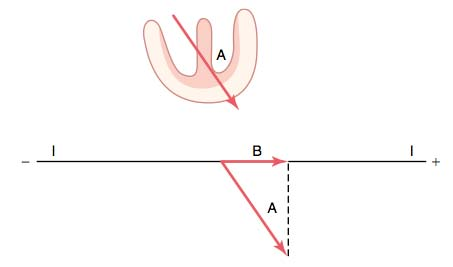
\includegraphics[width=0.7\textwidth]{../images/ECG_II_3.jpg}
\caption{Projection of the mean electrical axis onto lead I (vector B)}
\label{vector}
\end{figure}

\section*{Experimental Methods}
\subsection*{Electrode Placement}
\begin{enumerate}
	\item Place electrodes following the configuration for lead I:\begin{itemize}
		\item Red (+): left arm
		\item White (-): right arm
		\item Black (ground): right ankle
	\end{itemize}
	
	\item Place electrodes following the configuration for lead III:\begin{itemize}
		\item Red (+): left leg
		\item White (-): left arm
		\item Black (ground): right ankle
	\end{itemize}
	
	\item Plug leads I and III into channels 1 and 3, respectively.
	\item Open BIOPAC student lab lessons software and select \textit{Create/Record a new experiment}, and underneath it, \textit{Create empty graph} (Fig. \ref{menu}).
		\begin{figure}[h]
	\centering
\includegraphics[width=0.6\textwidth]{../images/ECG_II_9.png}
		\caption{Creating a new BIOPAC experiment}
		\label{menu}
		\end{figure}

	\item Select \textit{Electrocardiogram (ECG), 0.05 - 150 Hz} for channels 1 and 3 under presets, then check all the boxes for channels 1 and 3 (Fig. \ref{boxes}). Click \textit{Close} when you are done.
		\begin{figure}[h]
	\centering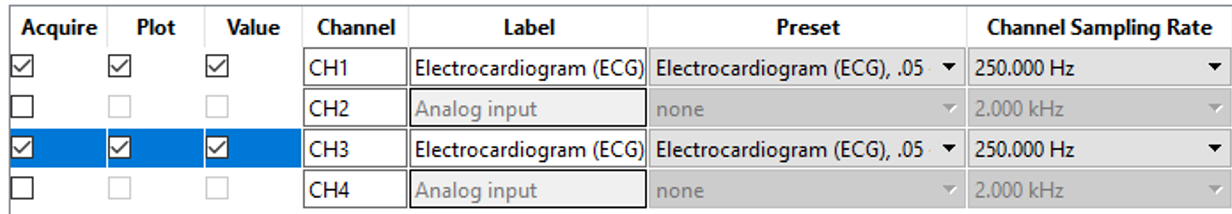
\includegraphics[width=0.6\textwidth]{../images/ECG_II_8.png}
		\caption{Select presets and check all the boxes for channels 1 and 3}
		\label{boxes}
		\end{figure}
\end{enumerate}

\subsection*{Data Collection}
You will perform data acquisition for four different conditions (supine, sitting up, inhaling, and exhaling). Calibration is not needed for this lab. Remember to insert markers to separate conditions, and to save the data file at the end.
\subsubsection*{Supine}
\begin{enumerate}
	\item Have the subject lay in supine position on a mat with eyes closed. Make sure the subject remains relaxed and still.
	\item Collect data for 20 seconds (press the green \textit{Start} button on the upper left hand corner).
	\item Click the \textit{Stop} button to pause or stop recording.
\end{enumerate}

\subsubsection*{Sitting Up}
\begin{enumerate}
	\item Have the subject sit upright in a chair. Make sure the subject remains relaxed and still.
	\item Collect data for 10 seconds.
	\item Click the \textit{Stop} button to pause or stop recording.
\end{enumerate}

\subsubsection*{Inspiration and Expiration}
\begin{enumerate}
	\item Have the subject remain seated.
	\item Collect data while the subject deeply inspires and expires, approximately 5 times in a period of 20 seconds.
	\item Place a marker after each inspiration and expiration, making sure to label them properly.
	\item Click the \textit{Stop} button to pause or stop recording.
\end{enumerate}

\subsection*{Data Analysis}
\begin{enumerate}
	\item Record the maximum electrical magnitude (amplitude) of the R waves for each condition for each of the two leads in the handout. Make sure the data corresponds to the correct lead number.
	\item Using data from the table, graphically determine the Mean Electrical Magnitude and Mean Electrical Axis for the conditions of Supine and Sitting Up. You may plot the values from both conditions on the graph on the handout.
	\item Explain the difference (if any) in the amplitudes of Leads I and III, as well as the Mean Electrical Magnitude and Axis under the two conditions.
	\item Using data from the table, graphically determine the Mean Electrical Magnitude and Mean Electrical Axis for the conditions of Inhaling and Exhaling. You may plot the values from both conditions on the graph on the handout.
	\item Explain the difference (if any) in the amplitudes of Leads I and III, as well as the Mean Electrical Magnitude and Axis under the two conditions.
	\item Give normal ranges of the mean electrical axis. Is your data within range?
	\item What factors affect the orientation of the mean electrical axis (list at least 2)?
	\item What factors affect the amplitude of the R wave recorded on the different leads (list at least 2)?
	\item It is unlikely your ECG data looks exactly like "textbook" data. List at least 3 sources of experimental error.
\end{enumerate}
\end{document}
